\section{Спектральное дифференцирование}

\subsection{Исходная функция}
Рассмотрим функцию $f(t) = sin(t)$ и соответствующий ей массив точек на промежутке $[-10, 10]$ с 
наложенным на нее небольшой случайный шум. График полученный функции приведен на рисунке \ref{fig:noised_sin}.

\begin{figure}[ht!]
    \centering
    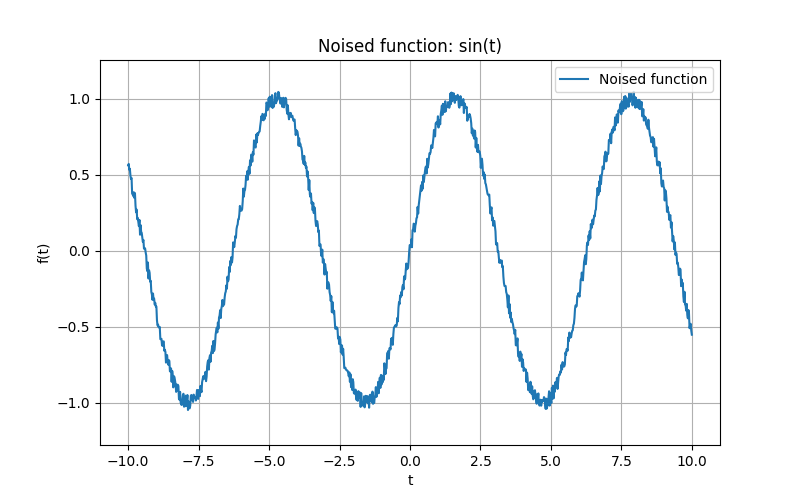
\includegraphics[width=\textwidth]{../results/10/noised_sin.png}
    \caption{Функция $f(t) = sin(t)$ с небольшим случайным шумом}
    \label{fig:noised_sin}
\end{figure}

\FloatBarrier
\subsection{Численная производная}
Найдем численную производную от зашумленной функции, используя поточечное дифференцирование: 
\begin{equation}
    f'(t) = \frac{y(k + 1) -  y(k)}{dt}
\end{equation}
график полученной производной приведен на рисунке \ref{fig:diff_noised_sin}.
На графике видно, что производная функции $f(t) = sin(t)$ с небольшим шумом также сильно зашумлена,
это связано, с тем, что значения исходной функции терпят сильные изменения за короткие промежутки времени.

\begin{figure}[ht!]
    \centering
    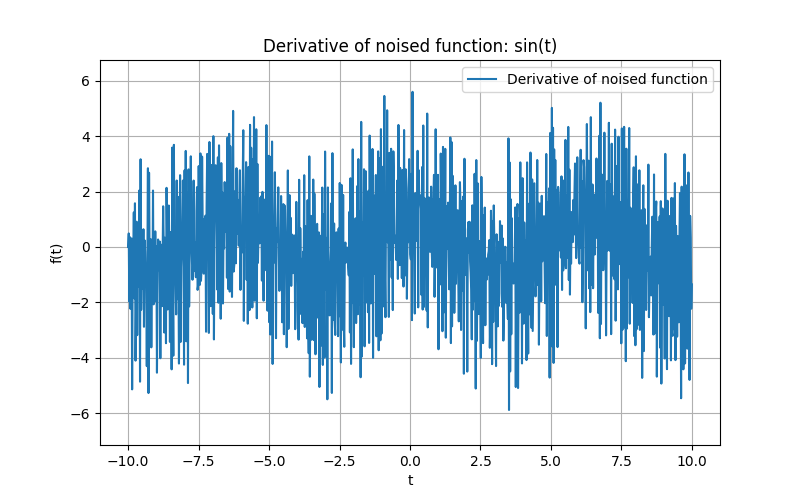
\includegraphics[width=\textwidth]{../results/10/noised_sin_derivative.png}
    \caption{Численная производная функции $f(t) = sin(t)$}
    \label{fig:diff_noised_sin}
\end{figure}

\FloatBarrier
\subsection{Спектральная производная}
Для нахождения спектральной производной найдем образ исходной функции $f(t)$ (см. рисунок \ref{fig:noised_sin_image}). 
\begin{figure}[ht!]
    \centering
    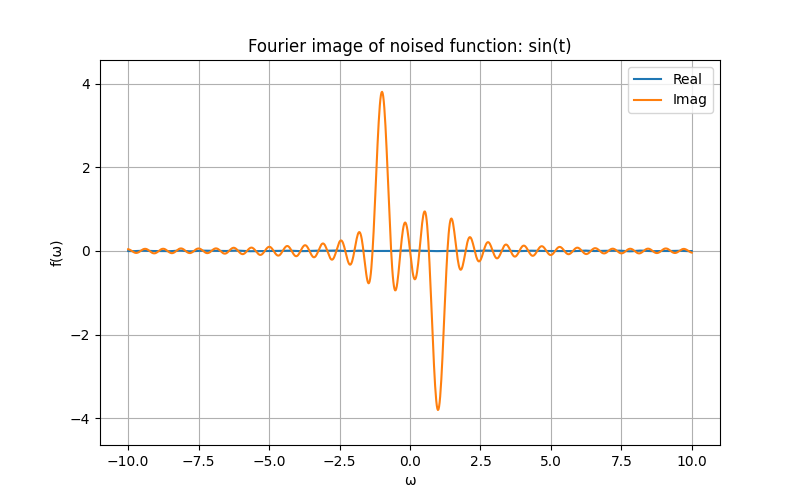
\includegraphics[width=\textwidth]{../results/10/noised_sin_image.png}
    \caption{Образ функции $f(t) = sin(t)$}
    \label{fig:noised_sin_image}
\end{figure}
Теперь, воспользовавшись тем, что:
\begin{equation}
    \mathcal{F}\{f'(t)\} = i \omega \mathcal{F}\{f(t)\}
\end{equation}
домножим образ функции на $i \omega$ и найдем обратное преобразование Фурье (см. рисунок \ref{fig:noised_sin_image_deriviate}).

\begin{figure}[ht!]
    \centering
    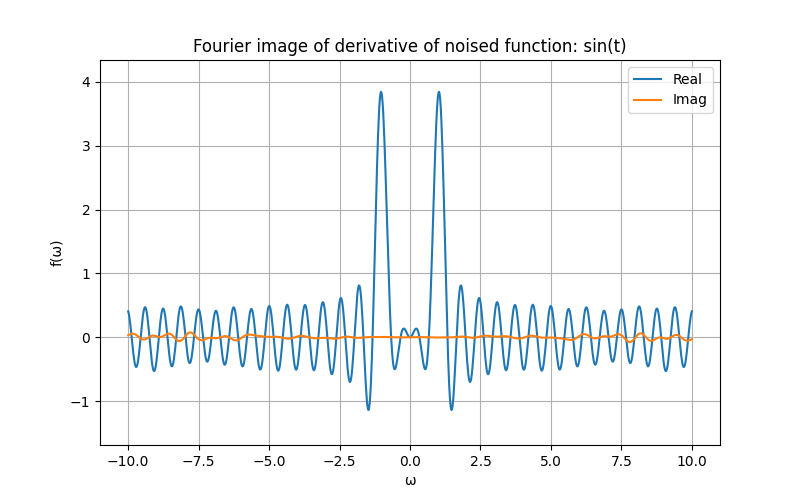
\includegraphics[width=\textwidth]{../results/10/noised_sin_image_derivative.png}
    \caption{Образ производной функции $f(t) = sin(t)$}
    \label{fig:noised_sin_image_deriviate}
\end{figure}
Найдем обратное преобразование Фурье от образа производной функции (см. рисунок \ref{fig:noised_sin_image_deriviate_restored}) и сравним его с численной производной и истиной производной $(cos(t))$ (см. рисунок \ref{fig:derivative_cmp}).

\begin{figure}[ht!]
    \centering
    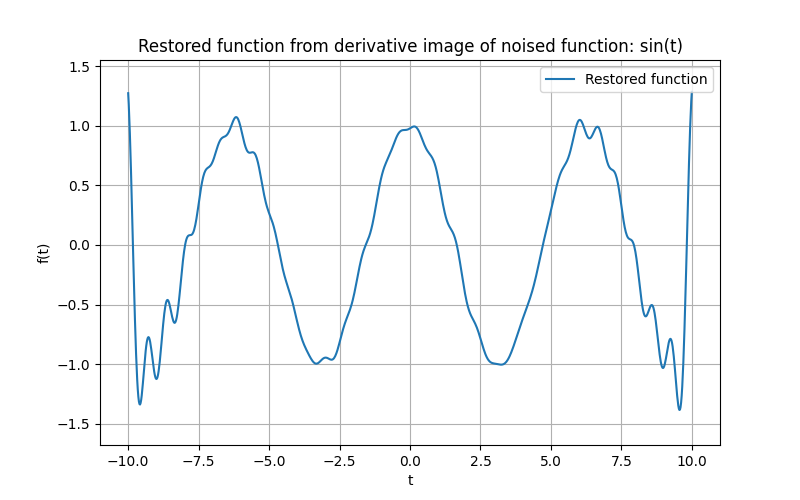
\includegraphics[width=\textwidth]{../results/10/noised_sin_image_derivative_restored.png}
    \caption{Обратное преобразование Фурье от образа производной функции $f(t) = sin(t)$}
    \label{fig:noised_sin_image_deriviate_restored}
\end{figure}

\begin{figure}[ht!]
    \centering
    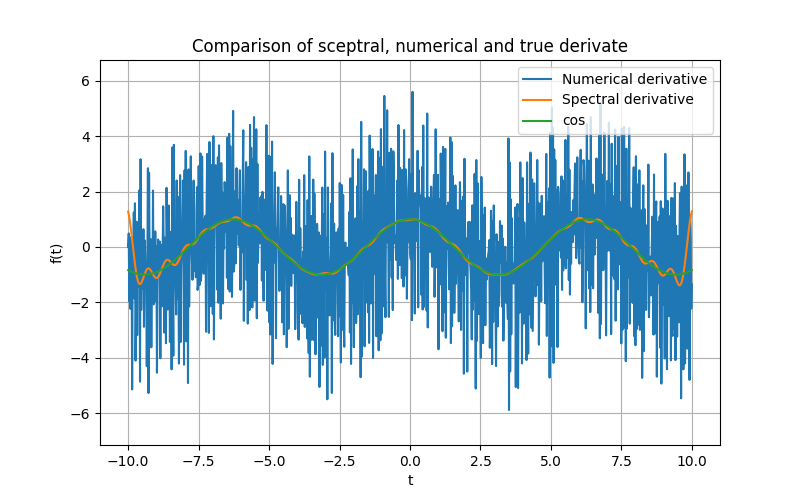
\includegraphics[width=\textwidth]{../results/10/derivative_cmp.png}
    \caption{Сравнение численной производной, истинной производной и спектральной производной}
    \label{fig:derivative_cmp}
\end{figure}

\FloatBarrier
На сравнительном графике (см. рисунок \ref{fig:derivative_cmp}) видно, что спектральная производная практически совпадает с истинной производной функции $f(t) = sin(t)$, в то время как численная производная сильно зашумлена и не совпадает с истинной.
Это, в первую очередь связано с тем, что при образ исходной функции $f(t)$ находился на промежутке $[-10, 10]$, а не на всей числовой прямой, что привело к фильтрации шума и улучшению качества производной. 

Графики для промежутка $[-100, 100]$ приведены в приложении \ref{app:A}, так как я посчитал их менее информативными и понятными. 